\section{Hardware Interface}
%Another flaw encountered regards the process of switching from the simulation environment to the real robot interface. As expected, even if the robot has been modeled and rendered almost perfectly for the simulation purpose, it lacks some important aspects of its dynamics.
\subsection{From Simulation to Real Robot}
The purpose of the development of robotics applications in a simulated environment is exactly to test and debug the software produced before loading it on the physical robot. To make this passage smooth and seamless, it has been implemented a hardware interface layer which provides an abstraction of the robot components, as shown in \autoref{fig:rosgazebointeraction}.
\begin{figure}[H]
\centerline{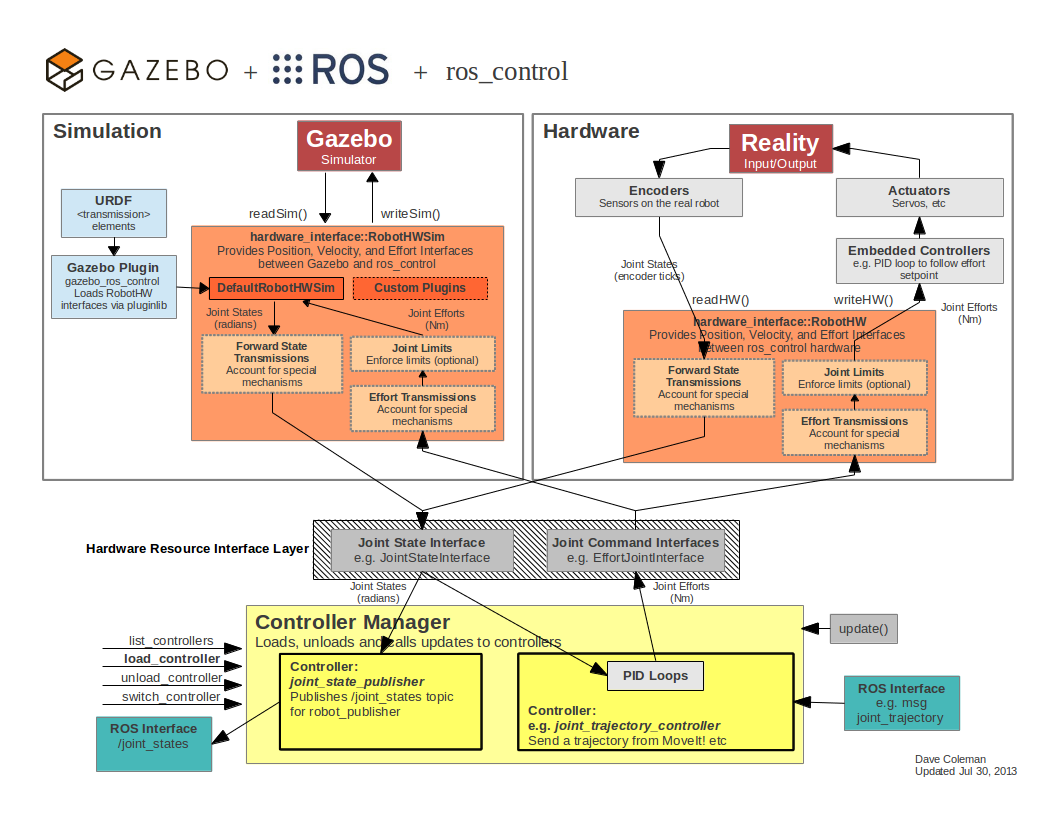
\includegraphics[scale=0.6]{ros+gazebo}}
\caption[Scheme of the interaction between ROS and Gazebo.]{Scheme of the interaction between ROS and Gazebo, with particulars on simulated and real robot.}
\label{fig:rosgazebointeraction}
\end{figure}
\subsubsection{Sensors Measurements (Joint State Interface)}
The major problem during the implementation regards the presence of sensors for joint velocities measurements. In fact, while Gazebo provides them accurately through simulated sensors, the KUKA LWR arm is only equipped with position and torque sensors. This, indeed, arises the need to derive the velocities from the measured positions through a process of online differentiation, with the following methods being analyzed
\paragraph{Euler Method}
This is one of the most basic techniques to compute numerical differentiation and its formulation is
\begin{equation}
\dot{q}_n = \frac{q_n - q_{n-1}}{h}
\end{equation}
where $h$ is the sampling time. Since the output of this differentiator is usually a bit noisy, it's convenient to pass it through an exponential smoothing filter, which is basically a weighted average between the last computed velocity value and the previous one
\begin{equation}
\tilde{\dot{q}}_n = \alpha\dot{q}_n + (1-\alpha)\tilde{\dot{q}}_{n-1} 
\end{equation}
where $\tilde{\dot{q}}$ denotes the smoothed value and $\alpha\in(0,1)$ is the smoothing factor.
\paragraph{Levant Robust Differentiator}
This method is based on the sliding mode theory and gives asymptotically exact derivatives \cite{levant06}. In comparison with Euler, Levant differentiator performs significantly better in terms of noise rejection and derivation of signals, but the major flaw which led this method to be discarded is that introduces a relevant phase shift.\\[1em]
So, according to the tests conducted and evaluating a trade-off between exact but out-of-phase signals and noisy but coherent signals, the best method resulted the Euler one.
\newpage